\documentclass{sbir}

\usepackage{fixme}
\fxsetup{
    status=draft,
    author=,
    layout=margin,
    theme=color,
    targetlayout=color
}

%%%%%%%%%% Proposal-specific Information %%%%%%%%%%%%%%%
\company{Modus Operandi}
\proposaltitle{GeoAID: Geographically-aware Assured Information Dissemination}
\topicnum{AF131-039}
\proposalnum{AF131-039-0xxx}
\proposaltype{SBIR Phase I Proposal}
%%%%%%%%%%%%%%%%%%%%%%%%%%%%%%%%%%%%%%%%

\begin{document}

\listoffixmes
\newpage
 
%%%%%  Roman numerals for TOC  %%%%%
\pagenumbering{roman}
\tableofcontents
\newpage
 
%%%%% Set the page number that the main proposal will start on %%%%%%
\pagenumbering{arabic}
 
\sbirsection{Identification and Significance of the Problem or Opportunity}
{The Modus Operandi Team proposes to develop geographically-aware assured information dissemination system called GeoAID.  This system will leverage our expertise and ongoing work in the areas of usage management and policy-based assured information sharing in network-centric multilevel security environments. The ability of GeoAID to rapidly and dynamically provide assured information and services to targeted devices within specific geographic regions will produce an information advantage for warfighters, and has direct commercial applicability to the emergency response industry.}
 
%%%%%  Evaluation Criteria box, use \begin{evalbox} \end{evalbox}, \evalhdr, \begin{evalitemize}, and \end{evalitemize}  %%%%% 	
\begin{evalbox}
\evalhdr{Innovative:}
  \begin{evalitemize}
     \item Addresses the GATSID problem via a proven and maturing policy-based usage management framework.
     \item Naturally incorporates location-based access policies into broader usage policies.
     \item Underlying logic framework supports sophisticated formal reasoning capabilities.
  \end{evalitemize}
\evalhdr{Sound Technical Approach:}
  \begin{evalitemize}
     \item Based on open standards and government off-the-shelf product development.
     \item Leverages UNM's demonstrated work in policy-based usage management.
     \item Leverages MO's proven work in knowledge management.
  \end{evalitemize}
\evalhdr{Qualifications:}
  \begin{evalitemize}
     \item MO Co-PI has significant experience with information assurance and knowledge management systems.
     \item AHS Co-PI has considerable expertise in information security and usage management in networked systems.
  \end{evalitemize}
\evalhdr{Benefits:}
  \begin{evalitemize}
     \item Dynamically and securely share information with properly credentialed users based upon their location.
     \item An agile usage management framework that scales to the enterprise level.
     \item Provides an information advantage to warfighters.
  \end{evalitemize}
\evalhdr{Commercialization:}
  \begin{evalitemize}
     \item Deployable in any networked environment where location-based usage policies apply.
  \end{evalitemize}
\end{evalbox}

\paragraph{Executive Summary}
\paragraph{The Problem.} The goal of this research and development effort is to build a system that addresses the Geographically-Aware and Targeted Secure Information Dissemination (GATSID) problem.  In the GATSID problem, the warfighter is assumed to possess an IP-based wireless device (or set of devices) that may connect to the military Internet. Furthermore, some collection of the devices associated with the network are assumed to support position location capabilities via GPS. Given these assumptions, the goal is to build a system that ``will enable on-the-move warfighters \ldots to securely send and receive information that can be targeted and tailored for sender-specified regions, sectors, or operating areas~\cite{AF131-039}.''  Given such a system, there are numerous scenarios (some of which are described below) where its capabilities could be leveraged to provide a distinct information advantage to the warfighter in the field. 

However, there are numerous difficulties with this approach that must be accounted for by any system deployed to address the GATSID problem.  Most importantly, all advantages to the warfighter may be lost if information is not delivered in a provably assured manner. Indeed, we can easily conceive of mission scenarios where opposing forces actually gain strategic advantage due to information leakage associated with an improperly designed location-based dissemination system.  It would not be difficult to build a system that addresses the GATSID problem if we could hold all aspects of the operating and mission environments constant. In this case, a set of rules for how and when information should be delivered to whom could be enumerated and exhaustively validated.  The reality, however, is that military network environments are constantly changing in ways that cannot be anticipated, and no two mission environments are the same.  Thus, an architectural framework that is overly rigid will lead to a system that cannot be easily adapted or scaled to address future needs.  It is not uncommon for the complexity of such systems to grow over time, leading to a security situation that becomes increasingly more difficult to manage.

\paragraph{The Solution Objective.} The Modus Operandi Team, composed of Modus Operandi (MO) and AHS Engineering Services (AHS), proposes to design, prototype and develop the Geographically-aware Assured Information Dissemination (GeoAID) system for addressing the GATSID problem.  The GeoAID system will be built on top of a highly flexible usage management framework that was designed to address situations very similar to GATSID, and was built with the notion of operating in Internet-scale environments involving highly complex usage policies.

\paragraph{Our Approach.} Our approach to developing the GeoAID is to leverage two critical information integration technologies, usage management and ...  focusing on the specific threat prosecution test case and dataset to be provided as GFI in Phase I.

\paragraph{Vision and End-State.} The end state of our Phase I research project will be the production of the GeoAID architecture and initial prototype that demonstrate the feasibility of our approach for success during Phases II and III. The methodology and prototype will be developed to support  the threat prosecution scenario provided by the government, in which we will demonstrate how operators configure the model to support their missions using the Operator's Tool. We will perform initial tests using the scenario data and measure results based on the usability and detect-to-engagement metrics. Finally, the \hl{gizmo} requirements, design, tool concept and metrics will be revised based on customer feedback. All results will be reported in the Final Technical Report and summarize in the Final Summary Report.
Our vision is to develop an intuitive, high-value \hl{gizmo} framework that can be integrated into the Air Force's  \hl{<blah blah>}. The specific products we propose to produce in Phase I, include:
\begin{itemize}
 \item A detailed \hl{gizmo} methodology and \hl{gizmo} requirements;
 \item An open, SOA-based \hl{gizmo} architecture and framework design that leverages the Wave-EF (unstructured data) and WebTAS (structured data) information integration frameworks;
  \begin{itemize}
   \item Design of extensions to Wave-EF technology needed to support \hl{gizmo} innovations:
   \item An \hl{gizmo} Threat Prosecution Knowledge Base consisting of the ontology, vocabulary and grammar needed to extract mission-relevant elements of information from text sources;
   \item A Mission-Specific RDF triple store that provides an archive of extracted and inferred knowledge for specific mission instances;
   \item An Operator's Tool that allows users to configure ASW F2F with the semantic structures required of their missions, to deploy and execute the software, and to provide human-in-the-loop inputs to the system during execution; 
   \item Services that provide external applications, such as USW-DSS, with access to ASW F2F services via a service bus;
 \end{itemize}
 \item A hybrid reasoning architecture that leverages appropriate statistical methods by data type, such as Bayesian Probability and Dempster-Shafer Theory for large amounts of hard (uncertain) data and inferencing rules (or logic) for soft data;
 \item An initial, highly focused \hl{gizmo} prototype to prove approach feasibility, identify critical research focus areas for Phase II, identify research issues beyond the scope of this effort, and identify tasks that can be automated and those requiring a human-in-the-loop;
 \item Metrics to determine operator usability and detect-to-engagement improvements;
 \item Documentation on the \hl{gizmo} methodology, requirements, architecture, and prototype;
 \item Required CDRLs, reports, and reviews, as well as professional publications.
\end{itemize} 

\paragraph{Background and Need}~\\
On the move warfighters require access to relevant, geo-tagged information. This information must be delivered to devices including handheld multi-function computers, either commercially available or militarized, or wearable computational systems incorporating novel user interface schemes.  

\begin{figure}
 \vspace{1in}
 \begin{center}
  $<$ A usage management figure goes here $>$
  \end{center}\fxfatal{Usage management figure}
 \vspace{1in}
  \caption{A high level depiction of the usage management framework.}\label{UM}
 \end{figure}

\sbircallout{The technical challenges.}{Current systems provide static, one-size-fits-all functionality for operational information delivery.  This is unsuitable for today's dynamic operational environments that change rapidly and unexpectedly.  Next-generation messaging solutions for the warfighter must incorporate dynamic security, innovative geo-tagged information dissemination, and the ability to adapt to chaotic technical operating environments.}

This kind of information can include textual data, video, audio, or any other kind of required data displayable on a range of devices within any number of applications, and will be  delivered to sender-specified geographic points or areas.  Devices are associated with specific geographic locations, and can receive messages that are pushed to them as needed, or statically posted at a specific region or point.  The system must support this kind of functionality globally, and maintain high performance under chaotic operational conditions.

\paragraph{Challenge 1: Eligible device capture.}  In order to effectively push notifications to eligible devices, those eligible devices must first be identified and captured by the system.  The overall system can capture these devices via pushing, polling, long polling, or some combination of these approaches.  Depending on the specific devices themselves, they may register themselves via other, underlying technical mechanisms as well.  Information must be transferred via internet protocol (IP), but certain devices like cell phones have other functionality of which this system can take advantage.  Furthermore, we have two distinct types of integratable devices.  The first, a fully featured device has IP networking capabilities as well as integrated global positioning system (GPS components).  This kind of device can be standalone and has an integrated sense of location.  The second device has IP networking capabilities as well, but uses geo-tethering to supply location services.

The local mechanisms supporting GeoAID are open ended with specific functional limitations.  Even though we have two specific device classifications the system must support, these device profiles need to be expanded to specific, phisical devices that may be used in the field.  Once identified, we can leverage these device's intrinsic applications and capabilities to provide a more integrated overall warfighter experience.  Other devices may be stripped down to only IP networking, installed application software enabling GeoAID, and either geo-tethered or native GPS services.  In either case, to minimize overall investment, we will use mobile-first development concepts to establish a common functional core that exploits other system services as they exists.

Likewise, overall device registration is can be implemented using a variety of different approaches.  Message delivery systems that push messages to registered devices have clear scalability advantages over polling-centric approaches, but are not always feasible to implement on limited systems.  An eventual production system may require a combination of pushing and polling, depending on clients and available services.  One of the goals of this work addresses how and why to combine these approaches most efficiently.

\paragraph{Challenge 2: Operational Scale.}  This kind of deployed system presents scalability challenges in a number of different ways.  Operational bandwidth may be limited, network latency may be high, and it is possible to have a large number of registered devices receiving messages in a small operational area.  The system as a whole will operate globally as well, requiring the ability to reliably distribute messages at internet scale.

Dynamic operating conditions my impose rapidly fluctuating network attributes.  This requires deployed systems to be able to smoothly adjust to changing conditions, including changes in available bandwidth.  This makes certain architectural choices more attractive than others.  Message pushing, for example, uses half the bandwidth as request/response based polling, but requires additional complexity on client and server systems.  Using appropriately scalable approaches is vital to providing appropriate in-theater levels of service.  Furthermore, approaches may need to change based on operating conditions.  In cases with high latency, devices may need to incorporate some kind of peering arrangement to facilitate timely notification delivery.

These kinds of problems are exacerbated by a pervasive internet-of-things.  As this kind of system moves from human-to-device to device-to-device modes of communication, possible supported information flow speeds, network requirements, and computational demands all increase.  These growing demands require innovative solutions supporting uninterrupted service under soft real-time constraints.

\paragraph{Challenge 3: Dynamic, secure information usage management.}  Delivering information securely over these kinds of networks requires a dynamic, adaptive approach to changing field conditions.  Information usage management in this environment depends on robust identification management, context dependent access control, and adaptive security primitives.

Any deployed system needs to understand who its users are and their attributes.  DoD has developed services supporting this kind of identification management (IdM) via deployed attribute services and role-based authentication mechanisms.  These same kinds of systems would need to be used operationally in order to evaluate information consumption suitability.

Access to information is heavily dependent not only on the person or device requesting or subscribed to data but also current operating conditions and intervening technology characteristics.  Under specific conditions, it may be in the interest of operating commanders to deliver information to individuals or devices that would not normally be allowed access.  These kinds of exceptional conditions, though rare, have certainly occurred in the recent past during natural disasters or unexpected enemy military operations.

Finally, wide availability of high performance computing components and advancing distributed algorithmics are rendering encryption based security approaches weaker and weaker.  Adaptive security systems that can dynamically route or redact sensitive information based on environmental conditions support new ways to protect information in motion.

\fxwarning*{Can we keep this?}{
\paragraph{Challenge 4: Warfighter Usability.}  Delivering information to and accepting updates from engaged warfighters requires a very small to non-existent cognitive load.  This implies nearly completely automated information collection and delivery systems which enable warfighters to focus on current operations while being able to access information when needed with little to no effort.

Though not completely in scope for this work, nevertheless deployed information delivery systems must be able to integrate easily from both a technical and operational perspective with deployed systems and personnel.  All developed systems must be able to integrate with sponsor standards to enable this kind of operational integration while supporting other, industry standards supporting technical system integration needs.}

\paragraph{Meeting the challenges.}  \fxfatal*{Content needed for meeting the challenges}{We need to flesh this out after completing the objectives section.}

\sbirsection{Phase I Technical Objectives}
{The project challenges motivate our technical objectives.  By meeting these objectives, we will develop a reusable architecture supporting geo-sensitive messaging for engaged warfighters, positioning this project for future phase II work.}

\paragraph{Objective 1: Device tracking.} Capturing suitable devices for receipt of sensitive broadcast information can take one of two general approaches, depending on the device type.  Devices can use either polling or registration models, either within the supported network stack or via other communications protocols.  The specific mechanism used depends on the class of device receiving messages.  While some devices only have simple IP-based communication available, other more sophisticated devices, like cell phones, may use alternative communication methods as well.

Polling models can be further sub-divided into polling and long-polling.  When simply polling, a device repeatedly contacts a known access point and passes required registration information to that access point.  The access point will then pass any information available and suitable for transmission to the requesting client.  The client will poll the access point repeatedly based on some established interval. That interval can change with each request, increasing or decreasing depending on the environmental context.   Long-polling, while superficially similar simple polling, does not close a connection after the initial poll.  The poll operation will block at the access point until any information is available to be transmitted.  When information does become available, it is sent to the client, which then immediately re-polls for additional information.  This essentially repeated registration for single message delivery.  These kinds of systems  pull information from an access point.

Registration models involve messages sent to endpoints known {\sl a priori}.  Registration can occur either at the application level, over the IP protocol, or via other network primitives available on the device.  Application-level registration is very flexible, and involves contacting an access point with information describing how to send messages to the device when required.  This kind of system is more complex than polling systems, but it will decrease the amount of traffic required to send messages to a given device.  In order to implement this kind of system, the client must be able to listen for messages. When implemented over HTTP, for example, this would require an HTTP server be available on the client.  In this case the client would register a URL with an access point.  The access point would then POST suitable messages to the URL associated with the client as those messages become available.  Alternative protocol registration behaves in a similar way, but the initial endpoint registration performed by the client is not over HTTP.  Rather, that initial registration takes advantage of an associated protocol.  Example protocols suitable for this kind of registration include control channel information over cellular standards like 3GPP LTE. Registration-centric systems involve data pushed from the client to the access point, and from the access point back to the client. 

Polling approaches all require an initial request for information, followed by a response.  Long-polling is more efficient that polling, as the response always has content and is never an empty response as long-polling blocks until content is available.  Registration methods use half the bandwidth of polling methods, generally, as information can be repeatedly pushed after a single registration.  In either case, mobile units will need to verifiably update location information regularly in order to ensure that appropriate geo-tagged messages can be delivered when available.

The final solution will require some combination of of these approaches, depending on the devices used and the robustness required.  Furthermore, under constrained operational conditions, client devices may need to use peer-based networking in order to effectively register, leading to further decreases in required bandwidth.  Our objective in this context will involve specifically extracting the optimal schemes for initial device registration for specific dynamic conditions, so that the system as a whole can operate as dependably as possible.

\paragraph{Objective 2: Operating at scale.} Distributing geo-sensitive information securely over today's active areas of operation requires adaptable systems resilient enough to support large volumes of devices with relatively low bandwidth.  Supporting these kinds of conditions requires intelligent systems capable of adjusting dissemination strategies in response to changing battlefield conditions.  Furthermore, the system itself will be a global DoD asset, requiring operation at internet scale.

Two common message-based architectures supporting these kinds of communication needs are hub-and spoke and mesh systems.  In hub and spoke systems, a single service point supports multiple clients.  These systems are easy to support and maintain, and straightforward to trace information through.  Information travels in a single hop from an access point to a client, with no intermediary.  Service functionality is clearly separated from client functionality as well.

Mesh architectures blend the boundaries between client systems and service providers.  In these configurations, clients can register with and receive information from access points or from nearby peers.  This kind of peer-to-peer communication would be hosted over IP at the application layer, and would serve to allow lower power devices access to GeoAID as well as potentially decrease the bandwidth requirements of transmitted messages.  The disadvantages of using this kind of configuration include additional client-side software complexity, non-deterministic message routing, and increased potential information exposure.  Clients must be capable of hosting and consuming services, leading to higher support requirements.  Furthermore, messages routed from peer system to peer system can be traced by logging system receipt but the number of hops is generally greater than one and is essentially unbounded unless an artificial hop limit is imposed.  These longer paths of transit for information lead to increased potential exposure as well, as a direct function of path length.

Further issues with scale arise when managing large numbers of registered devices.  Data systems supporting geo-located messaging must be able to process large numbers of registered client devices.  Timely delivery of messages delivered to a specific geographic area of interest at large scale requires advanced concurrent algorithmics capable of processing large numbers of similar data objects.  MapReduce algorithms fit this kind of scenario nicely, and would support the global scale required of this system.

Enabling operation in chaotic environments requires resilient systems capable of configuring themselves in response to changing conditions.  Fulfilling this objective leads to a system that can operate in both hub and spoke and mesh modes as environmental conditions dictate.  This flexibility, when coupled with robust information usage management, provides powerful and dependable geo-sensitive messaging.

\paragraph{Objective 3: Robust information usage management.} Information transmitted to registered devices must be secured via a variety of strategies.  Simple encryption based approaches, while necessary, are not sufficient to appropriately secure information.  Likewise, redaction-based schemes can prevent information from delivery to those who need it when then need it if inappropriately applied.

Appropriate usage management of included information is vital to maintaining confidentiality of sensitive data, but it must be applied dynamically in order to ensure appropriate information delivery.  Integrated information distribution systems that are able to take into account environmental dynamics as well as user and resource attributes while adhering to the spirit of sensitive data categorization can provide the appropriate level of control over information dissemination and use.

As an example, imagine a scenario in which a message containing specific medical information associated with personnel engaged in an upcoming high-risk operation fixed at a specific point in Afghanistan is placed by an analyst in Virginia.  This message is delivered to all registered and authorized devices within 10 miles of the message fixpoint.  The information in the message is very sensitive for the next 48 hours, after which it will be common knowledge.  Infrastructure between Virginia and Afghanistan is robust and reliable, and the message is secured by encrypted transmission over routes currently known to traverse friendly countries via the public internet.  Once the message arrives in Afghanistan, it is distributed via a mesh network to all appropriately authorized and known secure devices.  In this scenario, the information within the message is managed by the distribution system en route to Afghanistan, first. Here, the usage management system understands the dynamism of routing between Virginia and Afghanistan, and selects appropriately strong encryption as well as safe paths for the initial transmittal.  Once the message arrives in Afghanistan, the usage management system routes the messages to secure devices over secure mesh nodes based on the current conditions on the ground.  Once delivered, the information is restricted for the next 48 hours to specifically authorized personnel, after which it is made available to all registered devices so that they can appropriately support all personnel engaged within the operation.

In this scenario, the data itself is protected and managed at every step of it's transmittal and reception.  The usage of the information in the posted message has multidimensional protection at every step, and the usage of the information is managed after delivery as well.  This kind of responsive and aware usage management enables secure dissemination of dynamic data, providing information to those who need it most.

To meet this objective, we will incorporate our proven distributed usage management technology to provide flexible information protection.  We will incorporate this technology into the system holistically, providing a global umbrella of protection. 

\fxwarning*{The fourth objective; ease of use, focused on standards.  Do we want to keep this? If not we should delete the related challenge also and incorporate the ideas elsewhere.}{
\paragraph{Objective 4: Enhancing the warfighter.} ~\\
- non-interactive message delivery\\
- standards-based messages/systems for ease of system integration\\
}

%\fxfatal{This needs to all be updated with real content and objectives tied back to challenges.}{Our Phase I objectives focus on defining the ASW F2F methodology and architecture, as well as developing an initial prototype based on the government furnished threat prosecution scenario and dataset to demonstrate the technological foundation needed to support ASW F2F framework development in Phase II and subsequent Phase III commercialization. Since a comprehensive solution to the challenges introduced above is beyond the scope of a single STTR project, our overarching goals are to (1) develop the ASW F2F methodology, (2) design the ASW F2F architecture framework and (3) demonstrate the feasibility of evolving ASW F2F over time through the incorporation of new methods, capabilities and tools. Our specific technical objectives for the Phase I effort are discussed next.}

\begin{figure}
 \vspace{1in}
 \begin{center}
  $<$ A compelling high-level architectural graphic will go here $>$
  \end{center}\fxfatal{GeoAID architectural figure}
 \vspace{1in}
  \caption{GeoAIDS architectural overview.}\label{GeoAIDarch}
 \end{figure}

\sbirsection{Phase I Work Plan}
{This Phase I SBIR will result in the definition of the GeoAID technical approach and a software prototype that demonstrates the key aspects of our approach. These results will be in sufficient detail to show proof-of-concept and demonstrate feasibility for the Phase II project and Phase III commercialization.}
\fxfatal{Mark will add a work plan sentence here.}

\newpage 
\pagestyle{nonproprietary}
\paragraph{Phase I Work Plan Outline (Non-proprietary)}
\paragraph{Scope}~\\
The scope of this work is to build and deploy a system incorporating advanced usage management technology to securely delivery battlefield geo-aware updates to mobile warfighters.  Phase I work specifically addresses delivery a of a system capable of capturing eligible nodes and delivering appropriate messages to those nodes displayable on a geospatial display selected by a sponsor POC.  This includes delivery of supporting software code, documentation, and design artifacts.

\paragraph{Task Outline} 
\fxfatal{These need to match the tasks in the Tasks Details and Technical Approach section - Mark will fix.}
\begin{enumerate}
\item {\bf Kickoff Meeting} --- We will conduct a kickoff meeting with the project sponsor within 30 days of contract start.
\item {\bf Requirements Extraction} --- We will identify and enumerate system requirements, including identification of Sponsor POC geospatial technology.
\item {\bf Establish Approaches and Architectures} --- We will develop a catalog of architectural options including descriptions of the approaches and their advantages and disadvantages.
\item {\bf Evaluate System Architecture Options} --- We will examine the architecture options available and choose the most promising, as well as establish how a common extensible framework in which we can instantiate components embodying various approaches for future experimentation and comparison.
\item {\bf System Development} --- We will construct a simple framework, based on the common architecture identified in the previous task, which is relevant and applicable to the operational domain. We will verify that research components can be loaded into the framework and run correctly as expected to support the evaluation task.
\item {\bf System Evaluation} --- We will test the developed system and measure key performance attributes.
\item {\bf Technical Review Meeting} --- We will conduct technical review within six (6) months of project start at a date and time to be coordinated with the Sponsor POC.
\item {\bf Proof-of-Concept Prototype} --- We will develop a preliminary version of the GeoAID system as a proof-of-concept prototype demonstration using an accepted geospatial display from Sponsor POC recommended system(s).
\item {\bf Reports and Publications} --- We will write and submit monthly progress reports and a final report (with SF 298).
\end{enumerate}

\paragraph{Milestone Schedule}~\\
The proposed Phase I effort is scheduled as shown in the Gantt chart in Figure~\ref{Gantt}. The majority of the primary research will be accomplished during the first six months of the Phase I SBIR project. The last three months will provide project continuity to Phase II. Work will be performed at MO?s headquarters located in Melbourne, Florida, and at AHS Engineering Services facilities in Albuquerque, New Mexico.

\begin{figure}[h]
 \centerline{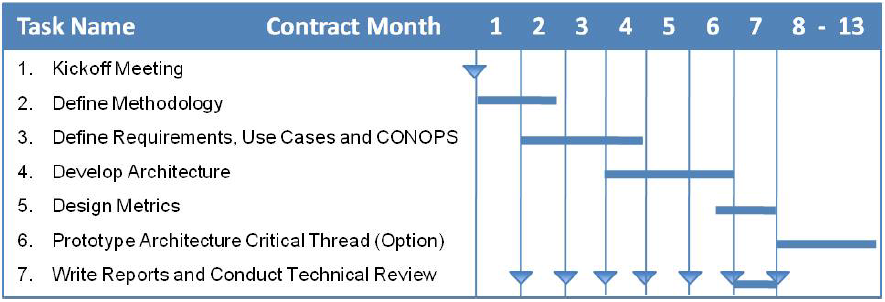
\includegraphics[width=5in]{./images/Gantt.png}}
 \caption{Task and Milestone Schedule.}
 \label{Gantt}
\end{figure}

\paragraph{Deliverables}~\\
We expect to have six specific deliverables as a result of this work.  These range from requirements documents to automated test suites to a deployable, operational system.
\begin{enumerate}
\item Kickoff meeting within 30 days of contract start.
\item Progress reports.
\item Technical review within 6 months.
\item Final report with SF 298.
\end{enumerate}

Our work plan is fully responsive to the requirements stated in the AF131-039 topic. By producing a working proof-of-concept prototype, we will in fact achieve more than the requirements of the topic.

\newpage
\pagestyle{proprietary}

\subsection{Key Aspects and Innovation}
Modus Operandi is an experienced and highly capable STTR/SBIR contractor with a proven record of thorough research and innovation, directed toward solving real problems. MO has been active for over a decade in researching the key technologies required in this effort. The University of New Mexico is a Carnegie Very High Research Activity University, and the Informatics Research Group is highly experienced in the areas of machine learning and hybrid intelligent systems. Our approach integrates proven existing technologies with new innovative approaches. The use and leverage of proven technology provides a sound foundation for our technical approach, reducing technical risk, and providing a platform for our key innovations.

\subsection{Task Summary and Schedule}
The proposed Phase I effort is organized into the tasks shown in the Figure~\ref{Gantt}. Work will be performed at MO's headquarters in Melbourne, Florida and at facilities in the Department of Electrical and Computer Engineering at the University of New Mexico in Albuquerque, New Mexico.

\begin{center}
\fcolorbox{BlueSteel}{Magnum}{
\begin{minipage}[t]{0.9\textwidth}
\begin{itemize}[labelindent=2em,leftmargin=1.5em,label=$\checkmark$] 
\item Building on information usage management and cloud expertise.
\item Reusing secure cross-domain information-centric systems for data delivery.
\item Mobile-first approach guarantees application-level configurability.
\item Innovative peering approaches to dynamic information delivery needs.
\end{itemize}
\end{minipage}}
\end{center}

\subsection{Task Details and Technical Approach}
The Modus Operandi Team proposes agile software development for accomplishing the Phase I tasks detailed below. Agile software development is a group of software development methods based on iterative and incremental development, where requirements and solutions evolve through collaboration between self-organizing, cross-functional teams. It promotes adaptive planning, evolutionary development and delivery, a time-boxed iterative approach, and encourages rapid and flexible response to change. It is a conceptual framework that promotes foreseen interactions throughout the development cycle~\cite{} \fxfatal{Add a good agile software development reference}

\heading{Task 1: Kickoff Meeting}
We will hold a kickoff meeting either at the government's site or at MO headquarters, in Melbourne, Florida, based on Government Sponsor Point of Contact (POC) preference. In this meeting we will review the proposed technical approach and statement of work and clarify the research sponsor's technical direction. In order to begin to address specific system needs, the team will assemble a coarsely grained Concept of Operations document that describes how the system should work. This will be a living document and will be updated regularly while the team executes other specific tasks. 

\heading{Task 2: Requirements Extraction}
The system has a wide requirements domain, stretching from dynamic information usage management to data storage to message delivery schemes. In this task, we will identify and enumerate system requirements, aiming for 90\% requirements coverage overall and 100\% requirements coverage with respect to core Phase I functionality. We will name and describe these requirements in a form suitable for future system development or documentation. This analysis includes identification of Sponsor POC geospatial technology used in future tasking.

The primary deliverable from this task will be a document describing these requirements such that the requirements can be traced both forward into the actual system and backward to the initial requirements source. The requirements will be enumerated as well as presented in either use case or user story formats.

\heading{Task 3: Establish Approaches and Architectures}
Capturing nodes suitable for broadcast is a difficult, nuanced problem. A variety of established architectural patterns can be potentially brought to bear on the problem, but they need to be carefully evaluated to ensure they will provide the required levels of service and scalability. In this task, we will outline the potential architectural approaches we can use, describe how and why they are applicable, and address how they could be evaluated for potential production use. We will leverage our established usage management technologies and experience to control information flow based on dynamic environmental context and used devices, extending that technology to seamlessly fit within this specific domain ~\cite{JaLaHe:11,JaLaHe:12}.

This task will result in the development of a catalog of architectural options including descriptions of the approaches and their advantages and disadvantages. This catalog will also include specific evaluation points and potential proofs-of-concept that may need to be built.

\heading{Task 4: Evaluate System Architecture Options}
Building on the catalog established in the previous tasks, we will evaluate outlined technical and architectural approaches with an eye toward identifying common features. We will examine the options available to us and choose the most promising as well as establish how we can establish a common extensible framework in which we can instantiate components embodying various different approaches for future experimentation and comparison.

The outcome of this task is an ordered listing of potential approaches and an architectural outline of a common framework in which we can test the approaches identified.

\heading{Task 5: System Development}
During this task we will build a simple framework based on the common architecture identified previously. We will keep the framework as simple as possible, but relevant and applicable to the operational domain. We will also develop components embodying the varied approaches to node capture, information usage management, and information dissemination. We will verify that these components can be loaded into the common framework and run correctly as expected to ease transition into future evaluation tasks.

We will further build upon our cloud engineering experience and in-house infrastructure to develop economical, standards-based systems based around portable system configurations. We will further automate event collection for future reporting using systems deployed in past information-centric data flow research~\cite{LaHe:12b}.

At the end of this task we will have source code available that is capable of loading the operational components on demand, as specified by previously identified configuration primitives. We will be able to load and run this system using accepted geospatial displays identified in previous tasks with the help of the Sponsor POC.

\heading{Task 6: System Evaluation}
At this point, we have established the key system components, developed the initial proof-of-concept technology, and are ready to evaluate various approaches and techniques. We will run the developed system during this task and measure key performance attributes like supportable system load, information delivery times, dropped messages, and appropriate message delivery. During this task, we will run the system and collect experimental results.

\heading{Task 7: Technical Review Meeting}
We will hold a technical review meeting with the project government sponsors within 6 months of project commencement. The GeoAID concept of operations, system requirements, and architectural options will be reviewed and refined at this meeting.

\heading{Task 8: Proof-of-Concept Prototype}
We will develop a preliminary version of the GeoAID system as a proof-of-concept prototype demonstration. We will provide the demonstration using an accepted geospatial display from Sponsor POC recommended system(s).

\heading{Task 9: Reports and Publications}
We will prepare monthly progress reports, the final technical report with SF 298, and the non-proprietary summary report, including all pertinent observations, nature of problems, positive as well as negative results, and design criteria established. We envision that one or more professional conference and journal papers will result from this research. With the customer's approval, we will publish the research results.

The tasks outlined within this proposal identify specific deliverables the team will develop and submit to sponsoring organizations. Those specific deliverables include:

\begin{itemize}
\item {\bf Requirements} --- A document listing identified requirements associated with requirement source organized both by list and context via use cases or user stories.
\item {\bf Architectural Catalog} --- A document describing system architectural options, advantages and disadvantages of those options, and how the they can be evaluated.
\item {\bf Software Source Code} --- Any and all developed source code, including proofs-of-concept and operational software.  This will also include documentation of the developed software.
\item {\bf Automated Test Suite} --- An automated test suite covering the system and all developed source code upon which the system is based.
\item {\bf Operational System} --- The operational system itself.  This will consist of associated hardware acquired for use, operating system images, source code, and deployment instructions, as applicable.
\item {\bf Final Findings Report} --- A report detailing the specifics of architectural evaluation activities, including information with respect to how the system operates, explanation of any design decisions made with supporting evidence, and guidance for future phase II activities.
\end{itemize}

\sbirsection{Related Work}{
Modus Operandi is highly qualified to successfully perform this effort based on our years of directly related experience in semantic technologies, data fusion, DOD ISR systems, and with enabling technologies such as service-oriented architecture and net-centric computing. AHS Engineering Services and the University of New Mexico's Informatics Lab are renowned for research in information security, information theory, and machine learning.}

\subsection{Co-Principal Investigators' Related Experience}
We propose Dr. Mark Heileman as MO's Phase I Co-Principal Investigator (Co-PI). Dr. Heileman has extensive experience as a research engineer and software system developer. His technological work has focused on applying artificial intelligence techniques and computer modeling to solve real-world business problems. Some of his early work in this area involved the practical application of expert systems and simulation modeling. More recently his work has involved the development of a trust evaluation framework for use in a layered sensing architecture that is intended to produce actionable situational awareness (the notion of trusted sensing is then built into the layered sensing architecture) [17; 18]. He is currently the Co-PI on both the SMASHUP Phase II SBIR project and the Nublu Phase I STTR project. The SMASHUP research project will result in the development of a formal framework that allows integration via mashups of content from various data sources in a secure manner [19; 20]. The Nublu research project will deliver technological innovations to provide assured information sharing (AIS) capabilities using flexible cloud computing based architectures. A summary resume for Dr. Mark Heileman is provided in Section~\ref{MDH}.
We propose Dr. Gregory Heileman as AHS's Phase I Co-PI. Dr. Heileman has over twenty years of experience as a research scientist, and has published over one-hundred peer-reviewed journal articles and conference papers. His research interests are in the areas of information security and multimedia systems, the theory of computing and information, and machine learning. He serves on the Editorial Board for the International Journal of Multimedia Intelligence and Security. Dr. Gregory Heileman is considered an authority on machine learning and information security [8]. He has published extensively in the area of machine learning, including research that dealt with the capabilities of neural networks, and he has proposed a number of neural network architectures and learning algorithms. Some of his early work in information security dealt with the development of secure container technology at the hardware level (see US Patent 6,731,756) [21]. His subsequent work has involved the development of architectural frameworks in support of access and usage control technologies [22; 23; 24; 25], information forensics [26; 27; 28], and semantics-based information valuation [10; 11; 12]. He is currently the Co-PI on the SMASHUP Phase II SBIR project and the Nublu Phase I STTR project; he will be a Co-PI on the ASW F2F Phase II STTR project. Dr. Gregory Heileman's experience is listed in Section~\ref{subs}.

\subsection{Modus Operandi Related Work}
Modus Operandi, Inc., is an advanced software technology firm serving the defense and intelligence community. We are focused on the development and marketing of technology and solutions that speed information discovery, integration, and fusion. We combine innovative semantic technology with defense sector software systems development experience in the Command, Control, Communications, Computers, Intelligence, Surveillance, and Reconnaissance (C4ISR) domain.

MO's R\&D focus is semantic web technologies with emphasis on semantic enrichment of multi-source data, intelligence fusion, unstructured information, reasoning, semantic integration, and migration of legacy systems to SOA. MO has deep expertise in text analytics, knowledge modeling and reasoning with heavy emphasis on open standards such as Extensible Markup Language (XML), XML Query Language (XQuery), RDF, SPARQL (recursive acronym for SPARQL Protocol and RDF Query Language),Web Ontology Language (OWL), and other semantic Web technologies. We pride ourselves on being a service-oriented company, adapting our wide background of in-depth experience to solve an extensive range of customer problems relating to information discovery and exploitation.

\subsubsection{Related Work -- Corporate R\&D and Phase III Commercialization}
{\bfseries Wave Exploitation Framework Technology Portfolio}---MO employs a portfolio commercialization strategy under a single brand, called Wave-EF, to achieve maximum payback for our investment in product management, marketing, and sales. An overarching portfolio roadmap and architecture integrates contributions from numerous SBIR/STTR projects, commercialization partners, and internal R\&D efforts. Wave-EF components are targeted at the challenges of processing multi-source intelligence for intelligence exploitation. Wave-EF performs ``semantic enrichment'' via text analysis and machine reasoning within a scalable, component-based architecture.

\subsubsection{Related Work -- Research \& Development}
Summarized below are the R\&D projects conducted by MO that address the critical technologies that will enable successful \hl{<blah blah>} R\&D.

{\bf Green Wave: Assuring Trust between the Edges Phase I SBIR}---This project dealt with the problem of delivering universal situational awareness to decision makers, and in particular with the problem of providing a means of quantifying the ``goodness'' of the various pieces of information contained within a layered sensing framework. Layered sensing is characterized by the appropriate sensor or combination of sensors/platforms, infrastructure and exploitation capabilities to generate that situation awareness and directly support delivery of ``tailored effects.'' During this research effort we created prototype architecture that supported the gathering and propagating (both forwards, for decision making, and backwards, for post mortem analyses) of ``trust information'' computed at various nodes in a network. In addition, we computed trust metrics from this information that could be provided to a decision maker. \emph{Contract Completed January 2009. Customer: AFRL/RYTC, Mr. Jong Hwang. (937) 255-4709 x3591}.

{\bf SMASHUP: A Formal Framework for Secure Mashups Phase II SBIR}---The recent development of mashup technologies now enables users to easily collect, integrate, and display data from a vast array of different information sources available on the Internet. The ability to harness and leverage information in this manner provides a powerful means for discovering links between information, and greatly enhances decision-making capabilities. The availability of such services in a DOD environment will provide tremendous advantages to the decision-makers engaged in analysis of critical situations, rapid-response, and long-term planning scenarios. In this research project, we have developed a framework that will allow integration via mashups of content from various data sources in a secure manner. The framework is based on mathematical logic wherein data units are wrapped in policies that provide rules over the manner in which information is collected, aggregated, and rendered in different environments. An advantage of this approach is it provides a formal means for controlling the usage of resources within highly complex secure mashups. \emph{Current Contract Awarded May 2011. Customer: AFRL/RIEBB, Mr. Matthew Shaver. (315) 330-3295}.

{\bf Nublu: Assured Information Sharing in Clouds Phase I STTR}---We are developing an assured information sharing framework for cloud-based systems that leverages our ongoing work in the areas of policy-based usage management and semantic interoperability. The development of this framework will involve the creation of a novel approach to information sharing that treats security as a commodity that can be dynamically provisioned within the cloud, along with other cloud resources. Currently, the security of networked infrastructures tends to be managed statically. That is, security requirements are developed and implemented within the networking environment, and all of the information that traverses the network will have these hard-coded security policies applied to it. The research project addresses this issue by logically separating security policies from security implementations within the network. This approach is vital if the true capabilities of the cloud are to be realized in DOD environments; it naturally meshes with the philosophy behind cloud computing. Specifically, the main advantage of cloud systems is the automatic provisioning of resources according to current demands. In a DOD setting there will be multiple missions currently interacting with the cloud infrastructure, and the proposed framework will allow each mission to do so according to the current security demands. \emph{Current Contract Awarded March 2012. Customer: AFRL/RITB, Ms. Virginia Ross. (315) 330-4384}.

{\bf Anti-Submarine Warfare Find-to-Forecast Phase I STTR}---The ASW F2F Project is focused on extracting situational knowledge from unstructured data sources, specifically tactical communications between Seahawk helicopters and the carrier, to fuse with structured data, such as radar and sonar data. This has involved developing a mission ontology for ASW, building a vocabulary for missions, and building specialized grammars for text parsing, tagging, extraction, and normalization as RDF triples. Phase I Contract awarded June 2011. \emph{Phase II Contract Pending Award. Customer: Office of Naval Research, Mr. David McGrane (360) 315-3531}.

\subsubsection{Related Work -- Technology Transition, Deployment, and Commercialization Opportunities}
This section summarizes the technology transition, deployment, and commercialization opportunities for Modus Operandi efforts relevant to the \hl{<blah blah>} project. Commercialization Partners are discussed in Section~\ref{commercialization}.

{\bf WebTHREADS}---MO's Wave text analytics and correlation technologies were integrated into the Web-based Threat HUMINT Reporting Evaluation Analysis and Display System (WebTHREADS), a web-based system for identifying and classifying intelligence reports used by Air Force organizations including the National Air and Space Intelligence Center (NASIC). Wave-EF uses domain-specific vocabularies, grammars, and ontologies to extract fourteen essential elements of information found in military intelligence reports, such as high-value individuals, locations, or events. MO also developed a tool for measuring the effectiveness of knowledge extraction from text, based on a standard text analysis metric, called F Factor Analysis. We plan to use this approach and these technologies to build up \hl{<blah blah>} mission vocabularies, ontologies, and grammars for  \hl{<blah blah>}  knowledge extraction, transformation, and normalization. \emph{Contract Completed December 2010. Customer: Air Force Electronic Systems Center, 630th Electronic Systems Squadron, Jonathon L. Cozad,  Lt USAF, (781) 266-0869}.

{\bf Air Force ISR Agency Semantic Analysis Tool (SAT)}---The AF ISR Agency sought to inject new technology for enhanced exploitation of multiple sources of unstructured data [further details classified]. \emph{Contract Completed December 2010. Customer: AF ISR Agency, Mr. John Gormaley (321) 494-0527}.

{\bf DCGS MC Multi-INT Semantics}---On this US Marine Corps project, Modus Operandi leveraged Wave-EF technology to build a DIB-enabled semantic wiki called Tactipedia. Tactipedia provides analysts with semantically integrated, mission-relevant information extracted from text sources. Links among pages (or semantic content) is based on semantic relations within an ontology, rather than hard-wired hyperlinks. In this way, Tactipedia's semantic model drives meaningful content integration as well as presentation to users. \emph{Phase II enhancement completed November 2011. Customer: USMC LtCOL Scott Camden, (703) 221-0200}.

\subsection{AHS Engineering Services Related Work}
Summarized below are the research projects conducted by AHS Engineering Services and the Informatics Research Laboratory at UNM that address the critical technologies that will enable successful \hl{<blah blah>} R\&D. As all aspects of science and society become increasingly information intensive, the need to understand, create, and apply new methods for modeling, managing, and acquiring information has never been greater. The UNM Informatics Lab, established by Professor Gregory Heileman, has considerable knowledge in the areas of information security, the theory of information, and information architectures [8].
~\cite{HeHeShGiJa:11,JaHe:08,JaHeLa:10,JaLaHe:11,LaJaBoNaHe:11,LaJaHeAb:11,LaHe:12,LaHe:13,PaSa:04,PuWe:02,SeKaBe:09,Co:09,Po:12}.

\subsection{State of the Art Related Work}
\fxfatal{Greg will provide an overview of usage management.}
\fxnote{This section is in progress; describing IP based geolocation, GPS integration, and GIS systems.}{
Current state of the art in location services for mobile device divides into a few distinct classifications.  On one hand, we have typical geolocation of mobile devices based on IP addresses.

Second, we have dedicated GPS systems with network links.

Though any of these systems can be used in device-to-device communication in a distributed internet-of-things, GPS-equipped units are more common as they can provide higher levels of geo-location granularity.

Finally, bringing this information together, we have data solutions like those embodied by Google Earth and ESRI products like ArcGIS.
}

\fxfatal{Is this real content for this proposal? I attempted to pull this into this document on a merge.}{
The art and science of multisensor data fusion has emerged as the foundation for the development of next generation net-centric decision support systems, including horizontal fusion systems. These decision support systems require the coordination of service-oriented sensors and fusion components. Distributed coordination-based architectures provide a process-to-process communications infrastructure that supports horizontal fusion services. In this paper, the author discusses architectural considerations for distributed service-oriented horizontal fusion including distributed coordination-based architectures, service access, data transformation, adaption, and end-to-end visualization [29].

Machine learning is concerned with the design and development of algorithms that take as input empirical data, from sensors or databases, and yield patterns or predictions thought to be features of the underlying mechanism that generated the data. A major focus of machine learning research is the design of algorithms that recognize complex patterns and make intelligent decisions based on input data. One fundamental difficulty is that the set of all possible behaviors given all possible inputs is too large to be included in the set of observed examples (training data). Hence the learner must generalize from the given examples in order to produce a useful output in new cases [30]. Numerous approaches have been developed ranging from neural network models to more abstract mathematical manipulations which identify numerical similarities. Nevertheless a common theme amongst the varied approaches is that learning techniques incorporate a strategic component to try and yield the best possible decision or classification. The mathematics of game theory formally analyzes strategic interactions between competing players and is consequently quite appropriate to apply to the field of machine learning with potential descriptive as well as functional insights. [7] authors present a game theoretic chip-fire classifier which is an iterated game that is able to perform pattern classification. [10; 11; 12] authors present a graphical-based model for explicit information valuation. The model caters to the subjective nature of information quality by measuring the impact a candidate piece of information may have on a knowledge base representing the recipient's world view. The model is capable of evaluating information semantically at the statement level and is in effect basing information-valuation on information-understanding. However, information value can be computed and predicted using the causal graph model without requiring full logical inference typically needed for information-understanding.
}

\sbirsection{Relationship with Future Research or Research and Development}{}
Modus Operandi was founded to address the practical application of innovative technologies. As a result, we are committed to the approach described in this proposal and are enthusiastic about its potential. The results of this program will have a significant influence on the future R\&D performed by Modus Operandi. Our work on data fusion, semantic interoperability, and machine reasoning efforts, such as SMASHUP, Green Wave, Nublu, and ASW F2F, provides an excellent technical foundation for the Phase I effort. Phase I will demonstrate the feasibility of our approach and will lay the groundwork for the Phase II development and transition. Specifically, upon successful completion of Phase I, we will have: (1) identified the critical aspects of our technical approach, (2) demonstrated the proof-of-concept, and (3) constructed a roadmap for application to Air Force initiatives such as AF DCGS (which includes identifying the applicable clearances, certifications, and approvals required to conduct Phase II testing). Collectively, the anticipated results from Phase I will provide a solid foundation for Phase II. In Phase II, we will build the full \hl{<blah blah>} framework and apply it to AF DCGS. Phase III would bring this \hl{<blah blah>} framework to the marketplace (see Commercialization Strategy below).
Our successful realization of our Phase I and II objectives and achievement of Phase III commercialization is expected to provide the following benefits to both Government and private sector customers of \hl{<blah blah>}:
\begin{itemize}
  \item Improve situation understanding with method and framework that focus on a specific mission to provide highly relevant results.
  \item Support machine learning and hybrid reasoning methods with extensible, open SOA architecture.
  \item Leverage legacy system investment with semantic interoperability.
\end{itemize}
We are confident of our ability to successfully deliver these benefits. As for future R\&D, we will seek out ways to extend the scope of \hl{<blah blah>} to include more sophisticated machine learning and reasoning capabilities.

\sbirsection{Commercialization Strategy}{Our overall strategy for achieving technology transition and commercialization success will be to position \hl{<blah blah>} as a high-value enhancement to our Wave product and related services, thereby leveraging our existing commercialization momentum and resources. Our three-pronged approach to achieving this strategy is to: (1) transition the \hl{<blah blah>} technology to AF DCGS, (2) deploy the technology to our other existing defense sector customers, and (3) leverage partnerships with prime contractors and commercial software vendors as channels for broader commercialization. Our overall goal is to build a profitable line-of-business while providing high return-on-investment to our Air Force transition customers.}
\label{commercialization}
\paragraph{Phase III Success Indicators:} 
\begin{center}
\vspace{-12pt}
   \fcolorbox{BlueSteel}{Magnum}{
         \begin{minipage}[t]{0.9\textwidth}
             \begin{itemize}[labelindent=2em,leftmargin=1.5em,label=$\checkmark$] 
  		\item SBIR/STTR Commercialization Achievement Index (CAI) of 90.
  		\item Annual corporate investment in commercialization initiatives exceeds \$1 million/year.
  		\item Winner of \$9.3M Phase III contract with Army CECOM in 2004 and \$9.9M Phase III in 2011.
  		\item Winner of U.S. Small Business Administration Tibbetts Award, recognizing our innovation, economic impact, and business achievements in the SBIR Program.
		\item Government prime contractor partnerships with Lockheed Martin, Northrop Grumman, ManTech, L-3 Communications, Booz Allen, SAIC, etc.
 	\end{itemize}
         \end{minipage}
      }
\end{center}

\paragraph{Background.} Modus Operandi's vision is to create solutions that speed information discovery, fusion, integration, and understanding. We combine innovative semantic technology with defense sector software systems development experience in the C4ISR domain. As demonstrated by our SBIR/STTR CAI of 90, we have a track record of successful technology commercialization, particularly with our Wave technology portfolio. Partly as a result of our SBIR/STTR commercialization and technology transfer efforts, our commercial (non-R\&D solutions for federal and private sector customers) business base has grown from less than 10\% to more than 60\% of our company's revenue. The following subsections provide our market analysis and plans for commercialization of \hl{<blah blah>}.

\paragraph{Commercialization Strategy.} Our experience has identified two keys to successful SBIR/STTR commercialization: (1) strategic synergy between the SBIR/STTR technology and our core business focus, and (2) strong Phase II/III partnerships.
This experience bodes well for the \hl{<blah blah>} project: first, because of \hl{<blah blah>}'s direct tie with our strategic focus on the intersection of semantic interoperability and fusion of multi-source information and the needs of the C4ISR community; and second, because the proposed application of the technology directly addresses challenges faced by the Air Force; by our other defense sector customers (i.e., US Army, Marine Corps, NAVAIR, Strategic Operations Command, and Missile Defense Agency); and by our prime contractor (e.g., Northrop Grumman, Lockheed Martin, ManTech, SAIC) and commercial (e.g., Ultra Electronics, Franz, NutraSpace) partners.
Our strategy for \hl{<blah blah>} commercialization will be as an integral part of our Wave product line and associated services. We plan to pursue three paths to commercialization of \hl{<blah blah>}. All of these paths are already part of our Wave marketing program.
\begin{enumerate}
  \item Our first path focuses on transitioning the technology to the AF DCGS thereby providing direct ROI for AFRL STTR investment. Our existing knowledge and experience working with the Air Force ISR Agency, the Electronic Systems Center, and the 45-th Space Wing will provide a solid foundation for success in this initiative.
  \item Our second path is deployment to our existing DOD customers and prime contractors, leveraging the \hl{<blah blah>} technology to address both known and anticipated needs they face in the area of machine learning and reasoning.
  \item The third path is expanding our business partnerships with prime contractors and commercial software vendors, increasing our market share in the federal sector, and ultimately taking us into the commercial marketplace. We are leveraging our partnership-building experiences to incorporate revenue channel and technology partnerships as a key element in our commercialization strategy.
\end{enumerate}

\paragraph{Market Need and Size.} Our commercialization strategy consists of two stages. We are currently focused on the first stage, which is establishing Modus Operandi as a premier niche technology solutions provider in the C4ISR market sector. The second stage will be to extend the business partnerships we develop in the first stage to package our Wave technology for the broader federal and commercial markets.
We are actively executing a comprehensive business plan which sets forth our strategy and roadmap for our technology, for delivering high value to customers, and for building a successful company. Our first stage market focus is on a niche within the \$16 billion C4ISR market [31]. Although overall defense-related spending is expected to flatten, and likely decline, over the next 10 years, the C4ISR market is projected for continued growth. The overall C4ISR segment is projected to grow at a compound annual growth rate of 2.98\% over the next decade [31]. This growth is fueled by the demand for timely intelligence as well as by technology and doctrine factors, particularly the demand for systems interoperability and the emergence of network-centric operations.
Within these overall market segments, relevant niche markets for Modus Operandi include Big Data, data discovery/integration/sharing, unstructured data analytics, multi-source intelligence analysis, and situational awareness, with concentration on the needs of U.S. DOD and intelligence community. Our preliminary estimate of the size of the MO-addressable portion of this market niche (comprised of R\&D, acquisition, and sustainment programs) is \$500-800 million annually.

\paragraph{Projected Commercialization Results.} Using our three-pronged strategy, we project achievement of the results shown in the Table~\ref{commercialization}. (Note: Our commercial market potential is not included, and offers the potential to significantly increase these estimates.)
\begin{table}
\begin{center}
 \caption{Actual and projected commercialization achievements.}\label{results}
 \begin{tabular}{|cccl|} \hline
  {\color{BlueSteel}\sf\bfseries\textsc Description}   &  {\color{BlueSteel}\sf\bfseries\textsc Timeframe} &    {\color{BlueSteel}\sf\bfseries\textsc Amount}  &  {\color{BlueSteel}\sf\bfseries\textsc Comments} \\ \hline
   Working Capital:  					& 						&						& Raised in April 2005 through sale of non- \\
   Funds Raised					& 			2005			&		\$450M			& core technology to a commercial firm.        \\
   Current Working Capital Assets		& 			2012			&		\$2M+			& Existing capital resources.                         \\ \hline
   Customer Investments (USAF 45th		&						&						& \$4.6M customer/investor funds and \$3M \\
   Space Wing, AFRL, AFTAC, AF		&		2004-2012		&		\$7.6M			& matching/add'l funds and CPP fund on       \\
   ESC, Marine Corps, CECOM and		&						&						& related Phase II SBIRs with USAF and        \\
   PEO IEW\&S)						&						&						& Army.						          \\ \hline
   Modus Operandi IR\&D Investment	&		2012-2015		& 		\$250K			& Estimated funds from additional Modus \\
   								&						&						& Operandi IR\&D investment.		          \\ \hline
   Additional Phase II/III 3rd-Party		&		2015-2016		&		\$2-3M			& Anticipated from early adopters and        \\
   Investment						&						&						& business partners.					\\ \hline
   Ramp-up Period Revenue			&		2016-2017		&	\$500K increasing 		& A 2-year ramp-up is projected. 		\\ 
   								&						& 	to \$3M annually		&								\\ \hline
   Full Scale Sales \& Marketing			&		2018 and 			& 	\$3+M annually			& Based on direct sales and co-marketing \\
   								& 		beyond			&	out of \$20M total		& initiatives. See assumptions below.	\\ \hline
 \end{tabular}
\end{center}
\vspace{-6pt}
{\small Key Assumptions: (1) Revenue includes both product licenses and related services. (2) MO participates as a partner in \$500 million of prime contractor/partner orders annually by 2018. (3) MO's revenue participation averages a minimum of 4\% (\$20 million annually by 2017). (4) The revenue share attributable to \hl{<blah blah>} is 15\% (\$3 million annually). (5) Excludes revenue from commercial markets.}
\end{table}

\sbirsection{Key Personnel}{Modus Operandi prides itself on teaming superbly qualified personnel for all of our projects. }
All key personnel are United States citizens. We propose Dr. Mark Heileman and Dr. Gregory Heileman as Phase I Co-Principal Investigators.  Dr. Mark Heileman's biography and r\'esum\'e are below. Dr. Gregory Heileman's biography and r\'esum\'e are in Section~\ref{subs}.
\begin{center}
\vspace{-12pt}
   \fcolorbox{BlueSteel}{Magnum}{
         \begin{minipage}[t]{0.9\textwidth}
             \begin{itemize}[labelindent=2em,leftmargin=1.5em,label=$\checkmark$] 
  		\item Dr. Mark Heileman has extensive experience as a research engineer and software system developer. He has focused on applying advanced information technology and modeling to solve real-world business problems.
  		\item Dr. Gregory Heileman is a recognized leader in machine learning and directs the Informatics Lab at the University of New Mexico where he is Associate Provost and Professor in the Department of Electrical and Computer Engineering.
 	\end{itemize}
         \end{minipage}
      }
\end{center}

\subsection{Modus Operandi Key Personnel Biography}\label{MDH}
{\bfseries Co-Principal Investigator. Dr. Mark Heileman} is a Senior Scientist at Modus Operandi. Dr. Heileman's over thirty-year career includes engineering and executive positions with Elisar Software Corporation, i2 Technologies, United Space Alliance, Rockwell International, and Harris Corporation. His mission is to focus on the client's challenges and employ a consultative, systems engineering approach to solve complex business needs. Dr. Heileman is a graduate of the University of Central Florida where he earned a Ph.D. in Industrial Engineering and Management Systems. He is a registered professional engineer in Florida.

\subsection{Co-Principal Investigator R\'esum\'e}
\textbf{\textsc{Mark D. Heileman \hfill Senior Scientist}}

\vspace{-18pt}
{\textcolor{black}{\makebox[6.5in]{\hrulefill}} 
\textbf{\textsc{Technical Expertise:}}
\vspace{-8pt}
\begin{multicols}{2}
 \begin{itemize}
  \item Enterprise Information Systems
  \item Digital Rights Management
  \item Cyber Security
  \item Expert Systems
  \item Data Aggregation
  \item Simulation and modeling	
 \end{itemize}
\end{multicols}
\vspace{-12pt}
\textbf{\textsc{Selected Publications:}}
\vspace{-8pt}
\begin{enumerate}
\item Heileman, M., G. Heileman, M. Shaver, P. Jamkhedkar, and M. Gilger. SMASHUP: Secure Mashup for Defense Transformation and Net-Centric Systems. Prepared for SPIE Defense, Security, and Sensing 2011 Conference, Orlando, FL, 25--29 April 2011.
\item Heileman, G. and M. Heileman. Method and Apparatus for Integrating Subjective Trust Measures into Automated Decision-Making Processes. Provisional Patent Application, USA, submitted 19 May 2010.
\item Heileman, M., G. Heileman, and J. Hwang. Integrating Subjective Trust into Networked Infrastructures. Prepared for Systems \& Software Technology Conference (SSTC) 2009, Salt Lake City, UT, 20--23 April 2009.
Hull, R., K. Bimson, M. Heileman, R. Hyle, and R. Thiebauth. Semantic Service-Oriented Architecture for Range Operations: Evolving the Role of Semantics in the Enterprise. Prepared for SPIE Defense, Security, and Sensing 2009 Conference, Orlando, FL, 13--17 April 2009.
\item Goldstein, H., G. Heileman, M. Heileman, et al. Protecting Digital Archives at the Greek Orthodox Archdiocese of America. Prepared for DRM'03, Washington, DC, 27 October 2003.
\item Linton, D., S. Khajenoori, M. Heileman, J. Bullington, H. Cat, K. Halder, G. Hebert, and S. Sinnappan. ``Reporter Object: An Analysis Module Which Aids in Verifying, Validating and Graphically Displaying Results of Simulation Models,'' Simulation, Vol. 62, No. 5, May 1994, pp. 313--328.
\item Heileman, M., D. Linton, and S. Khajenoori. ``Simulation Study Aids Space Shuttle Flight Rate Planning,'' Industrial Engineering, Vol. 24, No. 3, March 1992, pp. 58 --59.

\end{enumerate}
\textbf{\textsc{Relevant Experience:}}~\\
{\bfseries Modus Operandi, Inc., 2004--present. Senior Scientist.} A software company serving the US defense and intelligence community by providing technology to speed information discovery, integration, and fusion. Directs the design and development of innovative information system technologies and their application to government and industry needs.~\\
{\bfseries Elisar Software Corporation, 2001--2003. Vice President, Sales Engineering.} A venture capital financed start-up software company providing digital rights enforcement products and services. Initiated the Sales Engineering function, which had primary responsibility for driving customer and market requirements into the internal development process.~\\
{\bfseries i2 Technologies, 1997--2001. Senior Solution Consultant}. A business software and services company providing supply chain management solutions to customers worldwide. Provided technical leadership throughout software products sales cycles.

\textbf{\textsc{Education:}}
\vspace{-30pt}
\begin{tabbing}*****************\=\kill
 \> {\bfseries Ph.D.}, Industrial Engineering \& Management Systems, Univ. of Central Florida (1997). \\
 \> {\bfseries M.S.}, Engineering Management, Florida Institute of Technology (1990). \\
 \> {\bfseries M.B.A.}, Business Administration, Florida Institute of Technology (1985). \\
 \> {\bfseries B.S.}, Industrial and Systems Engineering, University of Florida (1980).
\end{tabbing}

\textbf{\textsc{Affiliations:}}
\vspace{-30pt}
\begin{tabbing}*****************\=\kill
\> Registered Professional Engineer, State of Florida (P.E. \#35539). \\
\> Senior Member, Institute of Industrial Engineers. \\
\> Member, International Council on Systems Engineering (INCOSE). \\
\> Security Clearance: DOD Top Secret/SCI/SI/TK/G/HCS.
\end{tabbing}

\sbirsection{Foreign Citizens}{}
We do not expect to involve any foreign citizens on this project.

\sbirsection{Facilities/Equipment} {}
All instrumentation and physical facilities required to carry out the Phase I effort are available at the Modus Operandi headquarters in Melbourne, Florida and at the University of New Mexico facilities in Albuquerque, NM. MO's 14,500 sq. ft. facility has a fiber optic Internet connection with a dedicated 4-Mbit bandwidth. Engineering laboratories host shared and project-dedicated resources, including two labs dedicated to classified work at the Secret level. These facilities meet all environmental laws and regulations of federal, Florida, and local governments for, but not limited to, the following groupings: airborne emissions, waterborne effluents, external radiation levels, outdoor noise, solid and bulk waste disposal practices, and handling and storage of toxic and hazardous materials.

\sbirsection{Subcontractors/Consultants}{Dr. Gregory Heileman and Dr. Chris Lamb are uniquely qualified for this effort, and their active involvement will ensure the success in delivering value to the Air Force Research Laboratory.}\label{subs}
{\bf Co-Principal Investigator. Dr. Gregory Heileman } is the Associate Provost for Curriculum and a Professor in the Department of Electrical and Computer Engineering at the University of New Mexico, with over 20 years of experience as a research scientist, and over 100 peer-reviewed journal articles and conference papers. At the University of New Mexico he teaches courses in the areas of algorithms and data structures, software design, theory of computing, learning theory, and information theory. His research interests are in the areas of information security and multimedia systems, the theory of computing and information, and machine learning. He currently serves on the Editorial Board for the International Journal of Multimedia Intelligence and Security. He is the author of the textbook Data Structures, Algorithms, and Object-Oriented Programming published by McGraw-Hill in 1996. During 1998 he held a research fellowship at the Universidad Carlos III de Madrid, and in 2005 he held a similar position at the Universidad Polit\'enica de Madrid. Dr. Heileman is a senior member of the IEEE. He holds a PhD in Computer Engineering from the University of Central Florida.

{\bf Senior Scientist. Dr. Christopher Lamb} will act as the primary Systems Architect during the course of all phases of the project. Dr. Lamb currently serves as an Enterprise Architect, with concentration on Systems and Security, with Sandia National Laboratories. He is also a research professor affiliated with the Electrical and Computer Engineering department at the University of New Mexico. He has extensive experience designing and developing mission-critical distributed systems for a wide range of government departments and agencies. Prior to joining Sandia National Laboratories, Dr. Lamb served in executive roles and as a principal consultant for a variety of technology companies in the southwest. Dr. Lamb has a B.S. in Mechanical Engineering from New Mexico State University, an M.S. in Computer Science from the University of New Mexico, as well as a Ph.D. in Computer Engineering with a focus on Computational Intelligence from the University of New Mexico. He is a The Open Group Architecture Framework (TOGAF) 9 Certified Enterprise Architect and a Certified Information Systems Security Professional (CISSP) through the International Information Systems Security Certification Consortium.

\textbf{\textsc{Gregory L. Heileman \hfill Professor and Associate Provost}}

\vspace{-18pt}
{\textcolor{black}{\makebox[6.5in]{\hrulefill}} 
\textbf{\textsc{Technical Expertise:}}
\vspace{-8pt}
\begin{multicols}{2}
 \begin{itemize}
  \item Machine Learning
  \item Usage Management
  \item Information Security
  \item Data Structures and Algorithmic Analysis
  \item Theory of Computing and Information	
 \end{itemize}
\end{multicols}
\vspace{-12pt}
\textbf{\textsc{Selected Publications:}}
\vspace{-8pt}
\begin{enumerate}
\item C. Vineyard, S.J. Verzi and G.L. Heileman.  Neurocomputation by a Neural Chip-Firing Game. Proceedings of the 2012 IEEE World Congress on Computational Intelligence, Brisbane, Australia, June 10--15, 2012.
\item C. Vineyard, G.L. Heileman, S.J. Verzi and R. Jordan.  Game-theoretic Mechanism Design Applied to Machine Learning Classification, Third International Workshop on Cognitive Information Processing, Baiona, Spain, May 28--30, 2012.
\item C. C. Lamb, P. A. Jamkhedkar, G. L. Heileman and C. T. Abdallah. Managed Control of Composite Cloud Systems. 6th IEEE International Conference on System of Systems Engineering (SoSE), Albuquerque, NM, pp. 167--172, June 27--30, 2011.
\item M. Martinez-Ramon, V. Koltchinskii, G.L. Heileman, and S. Posse. Classification of Multiple Interleaved Human Brain Tasks in functional Magnetic Resonance Imaging, in G. Camps-Valls, J. L. Rojo-Alvarez, M. Martinez-Ramon, editors, Kernel methods in Bioengineering, Communications and Image Processing, Idea Group, 2006.
\item S. al-Saffar and G. L. Heileman. Computing Information Value from RDF Graph Properties. Proceedings of the 12th International Conference on Information Integration and Web-based Applications \& Services, Paris, Nov. 8--10, 2010.
\item T.-T. Quach F. Perez-Gonzalez, and G. L. Heileman. Model-Based Steganalysis Using Invariant Features. IS\&T/SPIE Electronic Imaging Science and Technology: Media Forensics and Security XI (Conference EI120), San Jose, CA, Jan. 18--22, 2009.
\item S. al-Saffar and G. L. Heileman. Semantic Impact Graphs for Information Valuation. Proceeding of the Eighth ACM Symposium on Document Engineering, Sao Paulo, Brazil, pp. 209--212, Sept. 16--19, 2008.
\item S. al-Saffar and G. L. Heileman. Semantics-Based Information Valuation. Proceedings of the 4-th IEEE International Conference on Intelligent Systems IS'08, Varna, Bulgaria, Vol. 1, pp. 6-51--6-58, Sept. 6--8, 2008.
\item M. Martinez-Ramon, V. Koltchinskii, G.L. Heileman, and S. Posse. fMRI pattern classification using neuroanatomically constrained boosting. Neuroimage, 31(3):1129--1141, July 2006.
\item S. J. Verzi, G.L. Heileman, and M. Georgiopoulos. Boosted {ARTMAP}: Modifications to fuzzy ARTMAP motivated by boosting theory. Neural Networks, 19(2):446--468, 2006.
\end{enumerate}
\textbf{\textsc{Relevant Experience:}}~\\
{\bfseries AHS Engineering Services, 1997--present. Principal.} A consulting firm offering expert engineering services in areas including software engineering and information security.~\\
{\bfseries University of New Mexico, Department of Electrical \& Computer Engineering, 1990--present. Professor, Associate Provost for Curriculum (current position)}.~\\
{\bfseries Elisar Software Corporation, 2000--2003. Chief Executive Officer and Chairman of the Board.} A venture capital financed start-up software company providing digital rights enforcement products and services.

\textbf{\textsc{Education:}}
\vspace{-30pt}
\begin{tabbing}*****************\=\kill
 \> {\bfseries Ph.D.}, Computer Engineering, University of Central Florida (1989). \\
 \> {\bfseries M.S.}, Biomedical Engineering \& Mathematics, University of North Carolina (1986). \\
 \> {\bfseries B.A.}, Biology, Wake Forest University (1982).
\end{tabbing}

\textbf{\textsc{Affiliations:}}
\vspace{-30pt}
\begin{tabbing}*****************\=\kill
\> Editorial Board,  International Journal of Multimedia Intelligence and Security.  \\
\> Senior Member, IEEE. \\
\> Security Clearance: DOD Secret.
\end{tabbing}

\sbirsection{Prior, Current, or Pending Support of Similar Proposals or Awards}{}
No prior, current, or pending support for the proposed work.

 \bibliography{proposal}
 \bibliographystyle{abbrv}
 
 
 \hl{{\bf The Topic Call:} \\ The goal of the research and development effort is to build and demonstrate a software product called Geographically-Aware and Targeted Secure Information Dissemination (GATSID). GATSID will enable on-the-move warfighters, equipped with state-of-the-art wireless information appliances (e.g., handheld, commercially-available or militarized, or wearable computers), to securely send and receive information that can be targeted and tailored for sender-specified geographic regions, sectors, or operating areas. GATSID will enable mobile warfighters to rapidly react to changing battlefield conditions by delivering location-specific time-critical battlefield alerts and advisories. It will implement the following capabilities: 1. A geographically targeted information multicast service that enables an application to securely send data directed at mobile appliances situated within a specified geographic area. The area may be specified graphically (e.g., on a mapping display) or by identification label or geographic coordinates. A minimum of one point with operating radius or two or more points to define outer bounds of the affected area. 2. Range-restricted information dissemination service that delivers data securely to eligible mobile appliances within a given range (say 2 kms) of the information disseminator, where the latter could be a mobile wireless appliance itself. 3. ``Banner in the Sky'' service that allows information to be ``posted'' within a specified geographic region. The posted information is then delivered securely to any eligible fixed or mobile appliance entering the region. 4. Adaptation and customization of delivered information based on user's profile, user's device, and wireless link capacity. In the GATSID concept, the mobile warfighters are equipped with wireless information appliances such as smart phones that support two capabilities: 1) a position location mechanism (e.g., a Global Positioning Satellite [GPS]); and 2) an (Internet Protocol) IP-based wireless interface for connectivity to the military Internet. All communication to and from the mobile appliances is thus accomplished over IP. A non-GPS-equipped device may be referenced for another known GPS-equipped device(s). GATSID will address a major aspect of the challenge of delivering ``On-demand Information: ``What you need \ldots When you need it''. It will enable future situational awareness systems where intelligence and tactical sensor data must be exploited to provide customized, location-specific information to the force. The following paragraphs present example scenarios to illustrate the application of GATSID: Example 1: An unmanned aerial vehicle (UAV) operator performing a reconnaissance mission notices what appears to be a suspicious enemy activity in an area where Special Operations Forces (SOF) operations are ongoing. The pilot can use GATSID to send a targeted warning or alert message to all SOF warfighters in the vicinity of the threat. These warfighters will immediately receive this alert on their mobile appliances and can take necessary actions to counter the threat. Example 2: A first responder to an emergency uses his or her handheld device to broadcast a call for help to medical response teams within a 5 mile radius around the site. All medical 
response teams receiving the message can respond back with the ones closest to the site directed to proceed to the emergency scene.

PHASE I: Define, determine feasibility and demonstrate a means to collect and identify potential receiving nodes by class, location, or other means. Provide approach to capture the addresses (all modes) of identified receivers to provide multiple redundant alerts to the selected recipients. Provide demonstration using an accepted geospatial display from Sponsor POC (SPOC) recommended system(s).

PHASE II: Construct and demonstrate the operation of a prototype system utilizing one or more handheld devices currently approved for use by USAF or SOF warfighters. Demonstrate capabilities to alert nodes to action for response as well as action to head to safety. Working with the sponsor, utilize these capabilities in one or more approved experiments or exercises. 

PHASE III: Provide usability assessment of Phase II system for final user interfaces that will engage with existing receiver devices (minimum of 4--one sent from air operations center, one sent to/from SOF/embedded Joint Terminal Attack Controller or similar, and other vignette(s) determined in Phase II.
} 

 
\end{document} 